\section{STM32CubeMX og STM32CubeIDE}

\begin{frame}{Introduksjon}
	
\begin{figure}
	\centering
	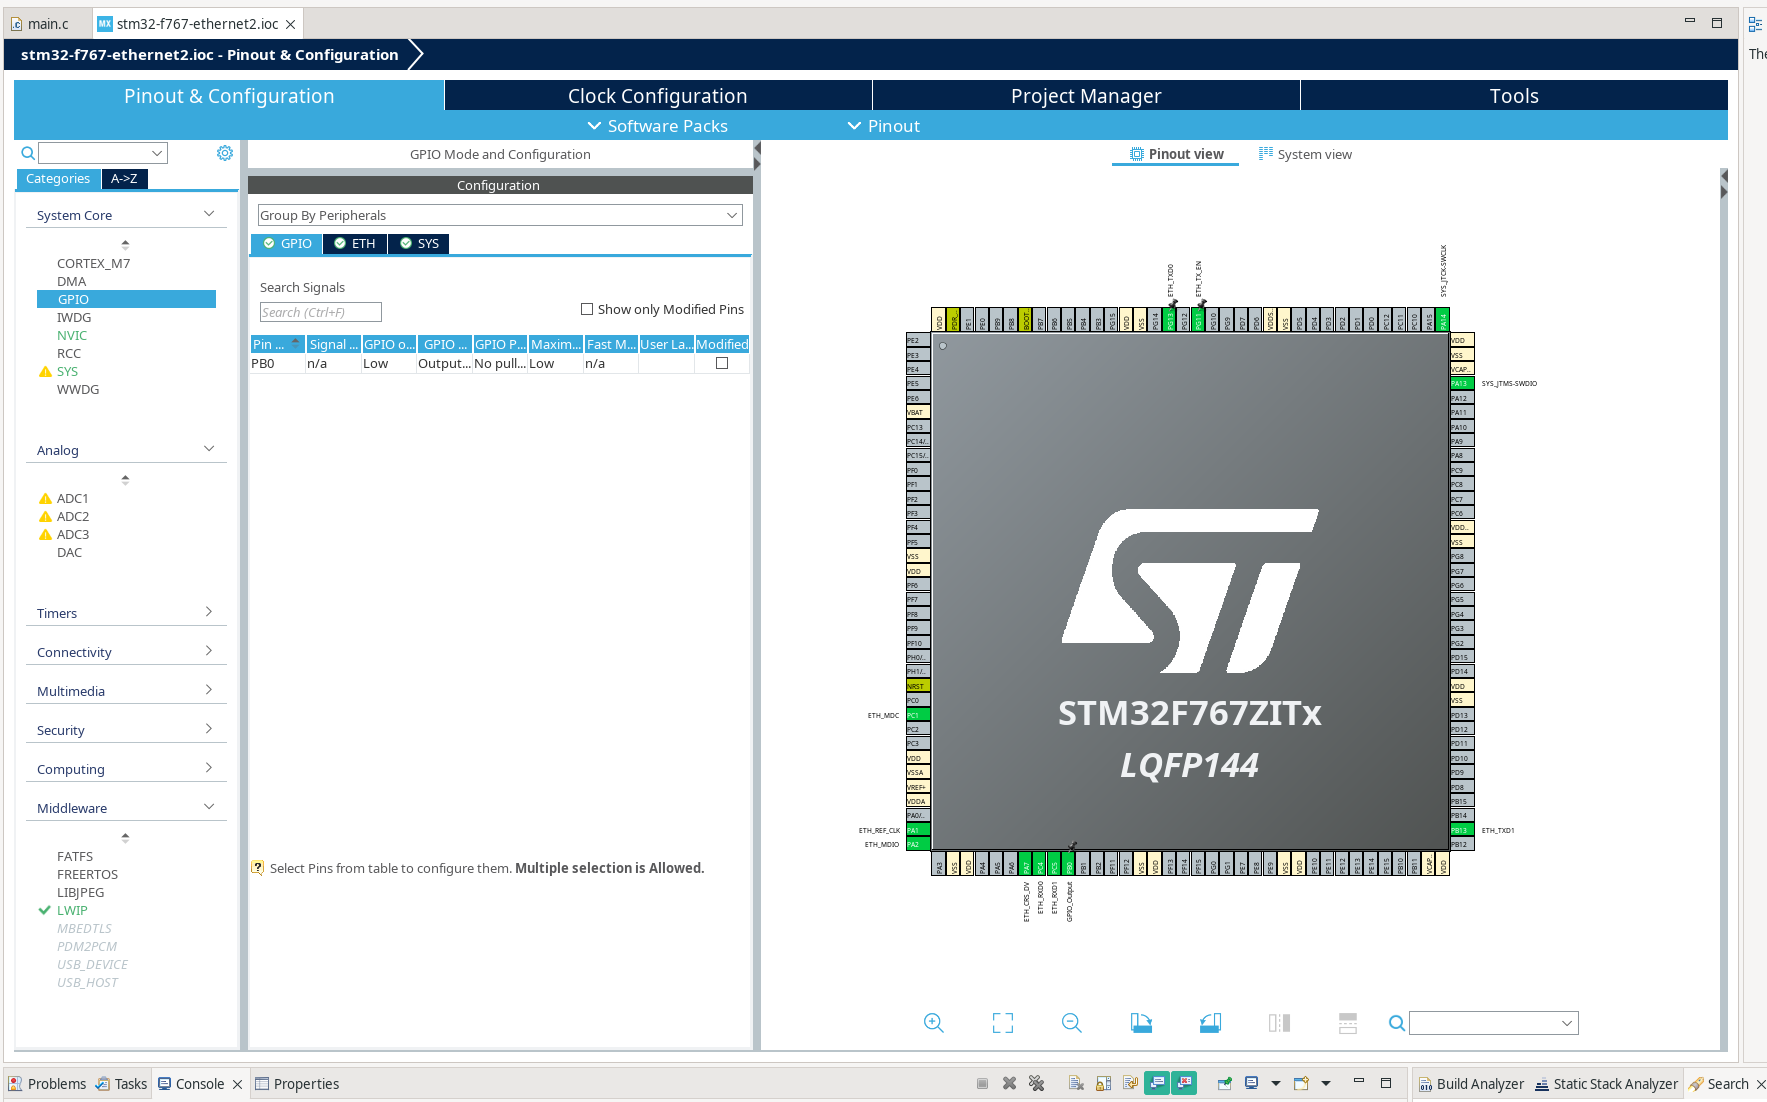
\includegraphics[width=0.9\linewidth]{img/stm32cubemx}
	\caption{Skjermbilete av pin-konfigureringa i STM32CubeMX}
	\label{fig:stm32cubemx}
\end{figure}

	
	
\end{frame}


\begin{frame}{Introduksjon}
	
	STM32CubeIDE er basert på Eclipse. Det er tungvindt å bruka, treigt og ustabilt. Det kan derimot vera nyttig å autogenerera delar av oppsettkoden for dei ulike pinnane på mikrokontrolleren ved hjelp av STM32CubeMX som kan nyttast som eit ``stand alone'' program, eller integrert i STM32CubeIDE.
	
	
\end{frame}
